\subsection{Pacchetto LoRaWAN}
\begin{figure}[h]
        \centering 
                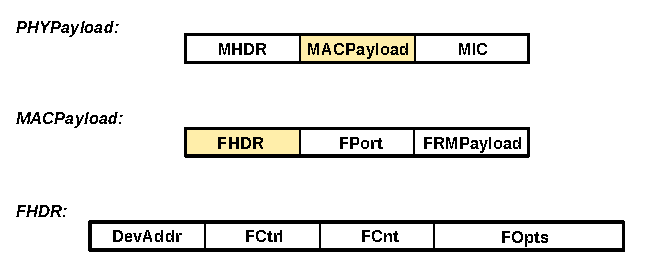
\includegraphics[width=11cm]{LoRaWAN_packet}
        \caption{Stack del protocollo della rete LoRaWAN}
        \label{fig:stack_lora}
\end{figure}
All'interno del frame \emph{PHYPayload} del pacchetto LoRa,  è contenuto il
messaggio LoRaWAN. 
Questo pacchetto è strutturato su due livelli,\ref{fig:stack_lora}.
Il MAC header contiene informazioni sulla versione dello standard usato nella
comunicazione, inoltre definisce il tipo di messaggio inviato, il quale può
esser di tre tipi
\begin{itemize}
        \item   \textit{Join packet}, cioè rappresenta la richiesta di un devices
                di entrare a far parte della rete.
        \item   \textit{Data message}
        \item   \textit{Proprietary message} usto per l'implementazione di
                messaggi non standard, utilizzabili per la comunicazione tra devices.
\end{itemize}
Il MAC payload contiene a sua volta il Frame payload, Frame port ed il Frame
header. Il Frame payload contiene al suo interno i dati inviati dall'Application
Layer ed il Frame port è utilizzato per determinare a quale applicazione il
messaggio è destinato, alcune di quest porte sono riservate per applicazioni
future.
